\section{Merchant}

\subsection{Managing products}
To manage the products on \textit{EmporioLambda} you must first access the merchant dashboard. To do so, click on the 'Merchant Dashboard' link in the header section of the website. You will then find a 'Product section' from where you can administer the listed products.

\begin{figure}[H]
\centering
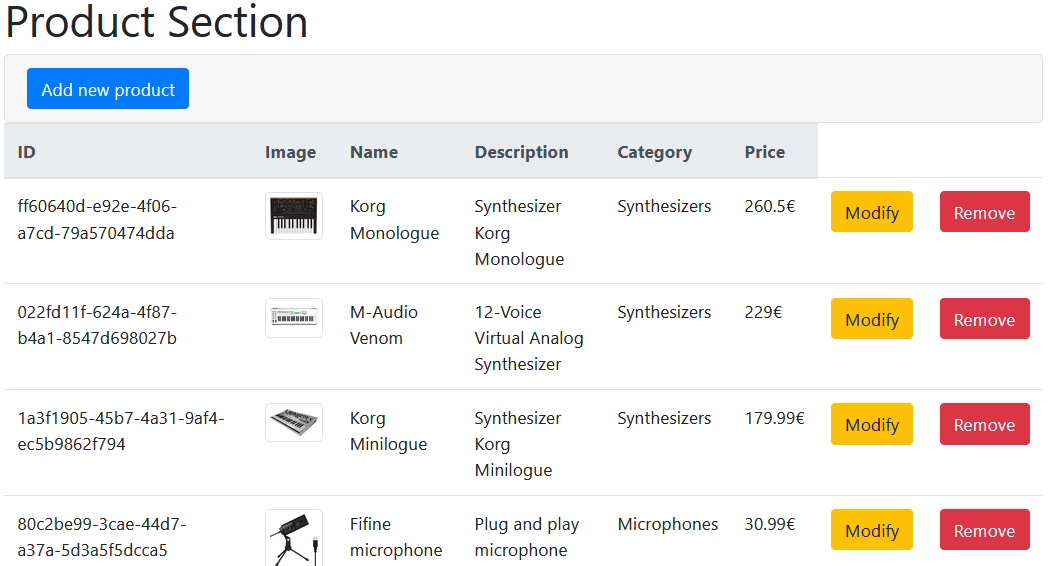
\includegraphics[scale=0.6]{res/Immagini/ProductSection}
\caption{Example of a merchant dashboard product section}
\end{figure}

From here you can add, modify or delete any product in the list.

To delete a product, click on the 'Remove' button next to it.

To modify a product's properties, click on the 'Modify' button next to the selected product. This will redirect you to a page with a form on which you will enter the updated data for the product. 

To add a new product, click on the 'Add new product' button. This will open a menu with a form to enter all of the necessary data. Clicking on the 'Submit' button will add a new product with the specified information.

\begin{figure}[H]
\centering
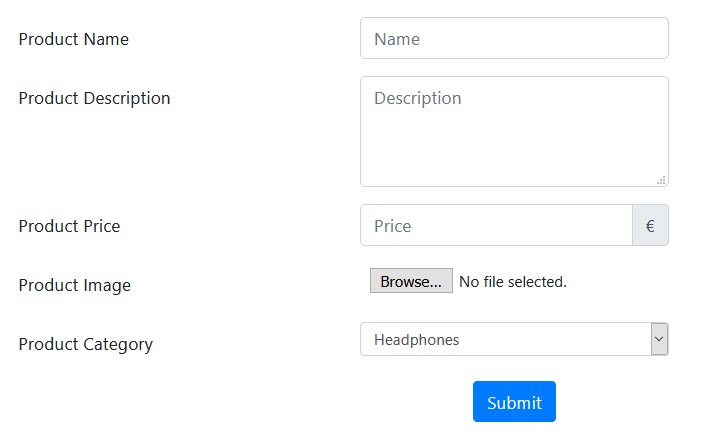
\includegraphics[scale=0.6]{res/Immagini/AddProduct}
\caption{Menu used to add a new product}
\end{figure}

\subsection{Managing product categories}
To manage the categories on \textit{EmporioLambda} you must first access the merchant dashboard. To do so, click on the 'Merchant Dashboard' link in the header section of the website. You will then find a 'Categories section' from where you can administer the product categories.

\begin{figure}[H]
\centering
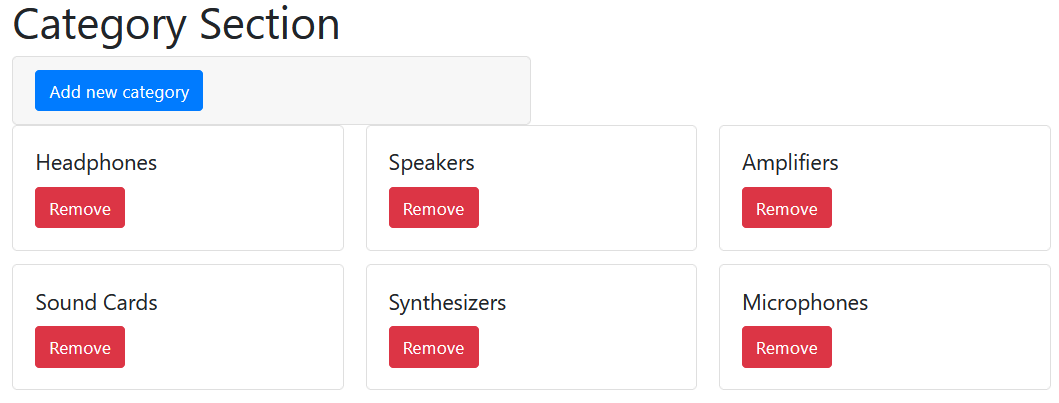
\includegraphics[scale=0.6]{res/Immagini/CategorySection}
\caption{Example of a merchant dashboard category section}
\end{figure}

From here you can add or delete the listed categories.

For a category to be deleted, no products must be using it. After making sure it is not linked to any products, click the 'Remove' button next to the desired category.

To add a new category, click on the 'Add new category' button. This will open a menu on which you can enter the name of the category. Pressing the 'Submit' button will add a new category with the specified information.

\begin{figure}[H]
\centering
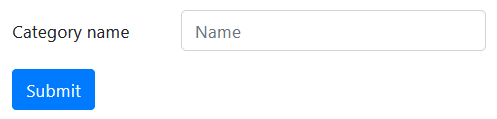
\includegraphics[scale=0.6]{res/Immagini/AddCategory}
\caption{Menu used to add a new category}
\end{figure}

\subsection{Updating the tax percentage}
To update the tax rate applied to all orders, open the merchant dashboard. You will find, under the category section, a 'Tax section' from which you will be able to update the current tax percentage. Simply update the value and click submit.
\begin{figure}[H]
\centering
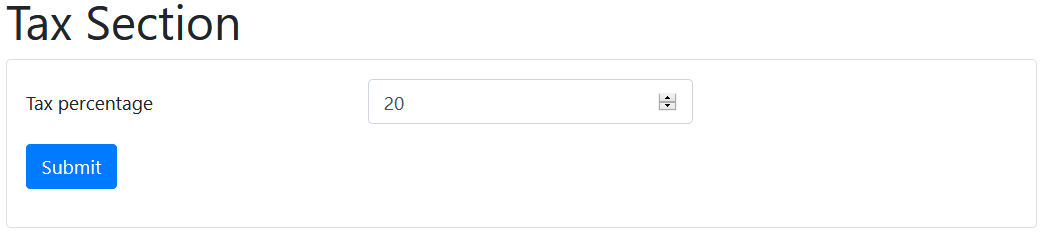
\includegraphics[scale=0.6]{res/Immagini/TaxSection}
\caption{Example of a merchant dashboard tax update section}
\end{figure}


\subsection{Accessing customer orders}
To access a list of all the received orders, navigate to the merchant dashboard. You will find, under the category and tax sections, an 'Orders section' containing all of the customers orders.

\begin{figure}[H]
\centering
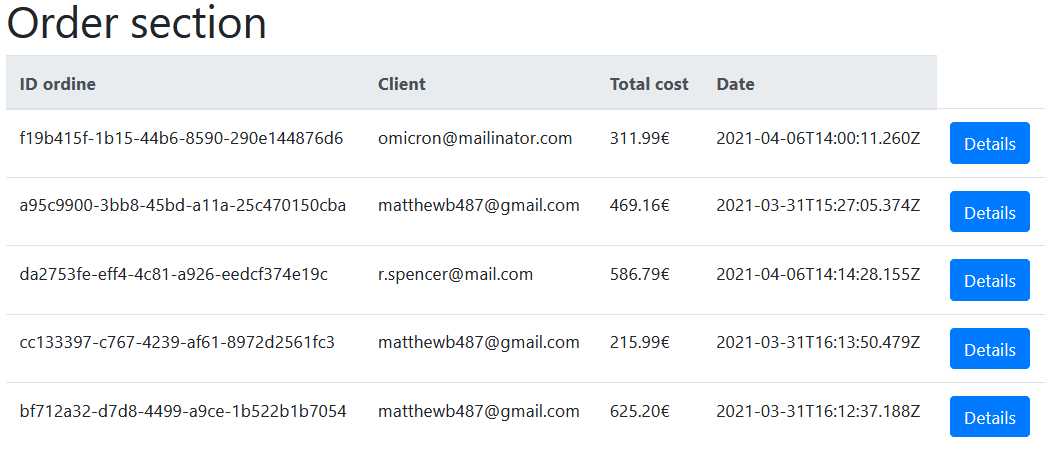
\includegraphics[scale=0.6]{res/Immagini/MerchantOrderList}
\caption{Example of a merchant dashboard order list section}
\end{figure}

To see more information for each order, click on the 'Details' button. You will be redirected to a page listing all of the order details.
